\section{Models}
With the question defined, the equations of motion derived, we can now consider the different models to achieve maximum displacement from a single jump.

% TODO: maybe put the constants before engine section
\subsection{Constants}
One might notice that I've deliberately left some of the constants $j_i$ clear of meaningful values and only suggested in-game default values. This is because many long-jumpers in the community find the default (vanilla) settings of the game engines ``bland'', reducing the excitement of this activity. Therefore, I will be setting some of the engine constants myself.

There are 4 of them:
\begin{itemize}
    \item \verb|sv_gravity| ($g$), set to 800
    \item \verb|sv_maxspeed| ($L$), set to 250
    \item \verb|sv_airaccelerate| ($A$), set to 10
    \item \verb|tickrate| ($n$), set to 64, or $\tau=\frac{1}{64}$
\end{itemize}

The only meaning deviation from the default settings are the speed limit $L$, for the default settings limits the optimization one can achieve, while the higher value of $250$ simply magnifies the result that one can achieve.

Furthermore, all models are free to set the initial velocity $\tv_0$, with the constraint that the magnitude of $\tv_0$ does not exceed $250$, the speed limit.

\subsection{Straight line}
% where you do nothing
We all know the fastest route (shortest distance) from point $A$ to point $B$ is with a straight line connecting $A$ to $B$. Therefore if the velocity magnitude is maximized, and as time is proportional to distance: $t = \frac{s}{\tmag{\tv}}$, it seems that a straight line would maximize the jumping distance assuming no constraints. This will serve as a good baseline for all the other models.

I have decided for the player to travel along the y-axis because I personally find it nicer to graph and draw with, but all maths would apply if you wish to substitute for the x-axis. This is represented by the acceleration function:

\begin{figure}[H]
    \centering
    \[
    \tunit{a}(t) = \tang{0, 1}
    \]
    \caption{The straight line model}
\end{figure}

Notice that player acceleration is constant in this model, and which can be achieved simply by looking forward, and press the key $w$ during the jump. Furthermore, we can set the initial velocity to point directly upwards in the y direction, such that:
\[
\tv_0 = \tang{0, 250},
\]
for common knowledge tells me that a faster initial speed in the direction where I am going will result in higher overall travel distance. Overall, there exists four metrics for each model, each worth evaluating.

We can first look at the case without the max speed constraint. By running a simulation with the engine constants discussed before, I got a result of $\approx 807.5$ hammer units in a jump. Predictably, this model will have the player traveling in a straight line (figure \ref{fig:straight_nothing_1}).

\begin{wrapfigure}{r}{0.48\textwidth}
    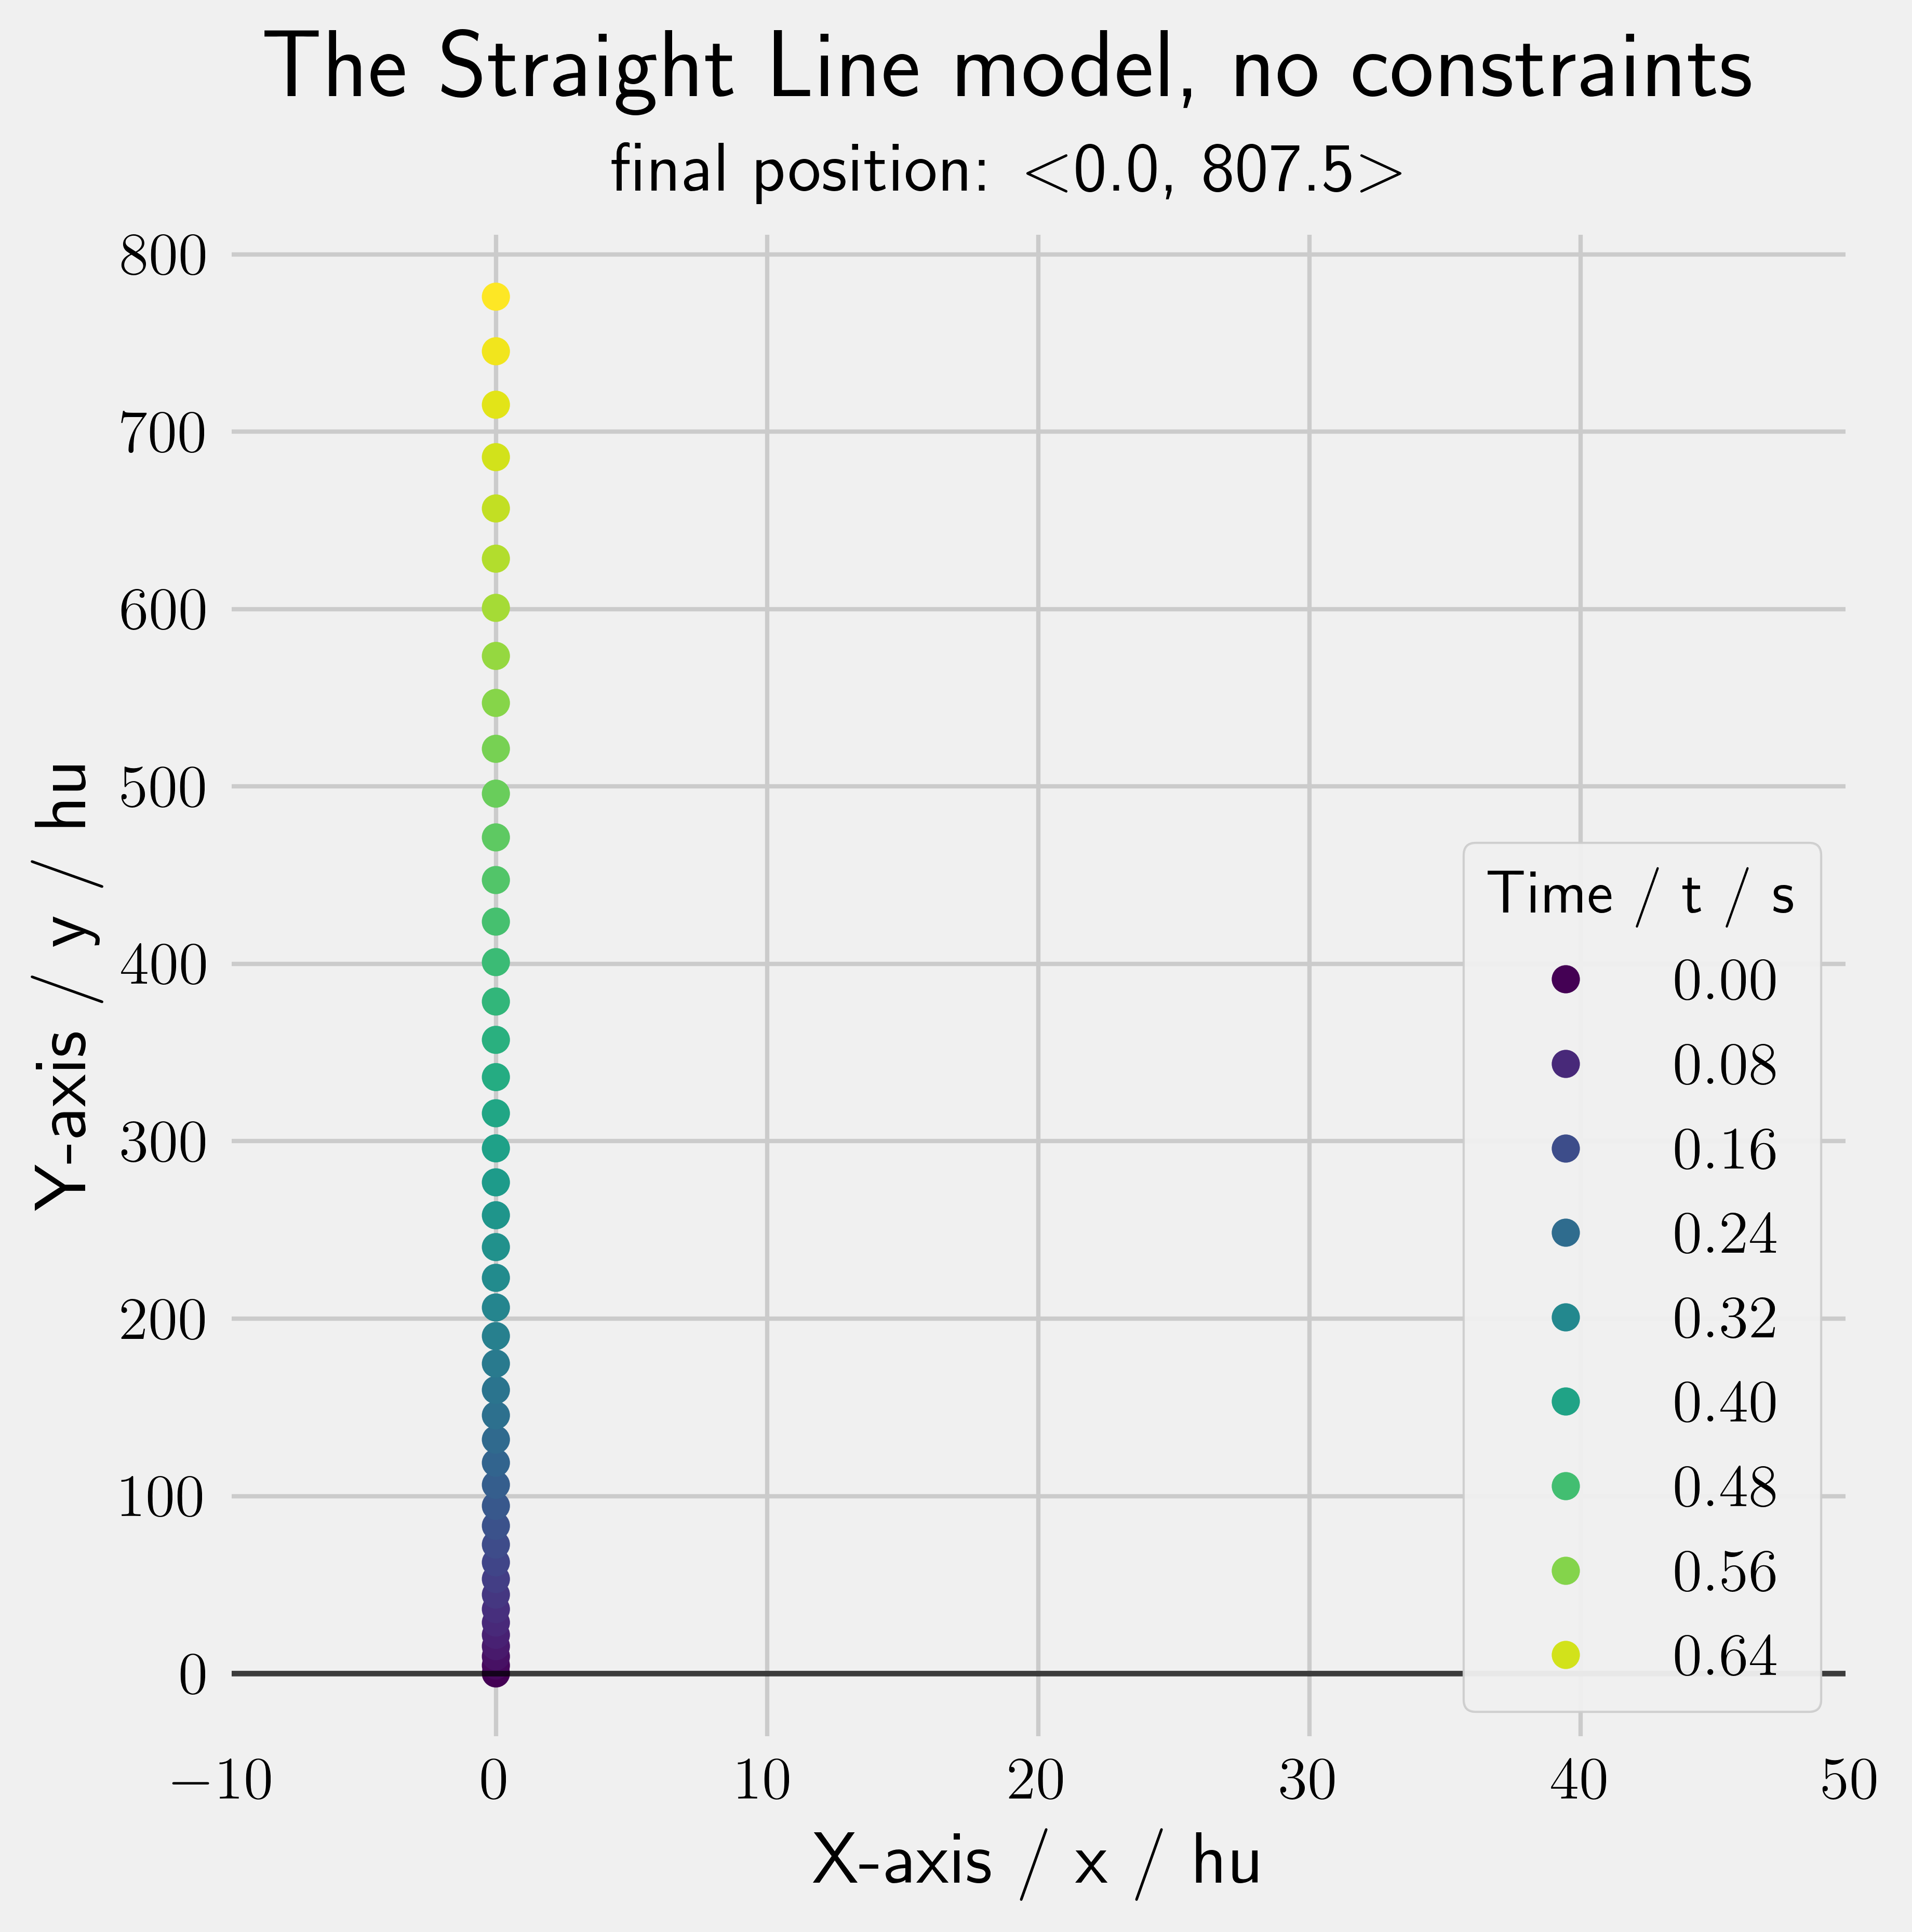
\includegraphics[width=0.45\textwidth,right]{assets/straight_nothing_1.png}
    \caption{}
    \label{fig:straight_nothing_1}
\end{wrapfigure}

I can comfortably say that this jumping distance would never be possible to achieve in game, for this model can be proven to be the most optimal jumping path if there are no speed limits (appendix, using EL equation). This number of around $800$ hammer units serves to be the upper-bound output of our optimization, and the lower-bound being its negative of around $-800$ (if you wish to accelerate directly backwards with negative initial velocity).

Additionally we can also utilize the equation derived in the last section (equations \ref{eq:jumping}).

Using the acceleration function, we can define $x(t)$ and $y(t)$ as:
\[
    x(t) = 0, \quad y(t) = 1.
\]

Their first and second order indefinite integrals can be obtained using calculus:
\begin{alignat*}{3}
    X(t) &= \int x(t) \, dx = 0, \quad
    &&\tfx(t) &&= \int X(t) \, dx = 0\\
    Y(t) &= \int y(t) \, dx = t, \quad
    &&\tfy(t) &&= \int Y(t) \, dx = \frac{1}{2} t^2,
\end{alignat*}
notice that the constants during integration are omitted as we've incorporated them into the derivation of the jumping motion equations as $c_1$, and $c_2$.

Therefore the $x$ position after $t_f$ seconds assuming no speed limit is:
\begin{align*}
    p_x &= p(t_f)_x = w\tfx(t_f) + t_f(v_{0x} - w\tfx'(0)) - w\tfx(0)\\
    &= w \times 0 + t_f(0 - w \times 0) - w \times 0\\
    &= 0,
\end{align*}
and the respective $y$ position is:
\begin{align*}
    p_y &= p(t_f)_y = w\tfy(t_f) + t_f(v_{0y} - w\tfy'(0)) - w\tfy(0)\\
    &= w \frac{1}{2} t_f^2 + t_f(v_{0y} - w v_{0y} \times 0) - w \times 0\\
    &= (10 \times 250) \frac{1}{2} (0.7)^2 + 0.7 \times 250\\
    &= 787.5
\end{align*}

% TODO: change A to 10

The jumping motion differential equations resulted in a similar sized jumping distance in comparison to the engine simulated $\approx807.5$. I believe that a $\frac{|787.5-807.5|}{807.5} \approx 2.48\%$ error is a very well approximation of this continuous method for future modeling.

\begin{wrapfigure}{r}{0.48\textwidth}
    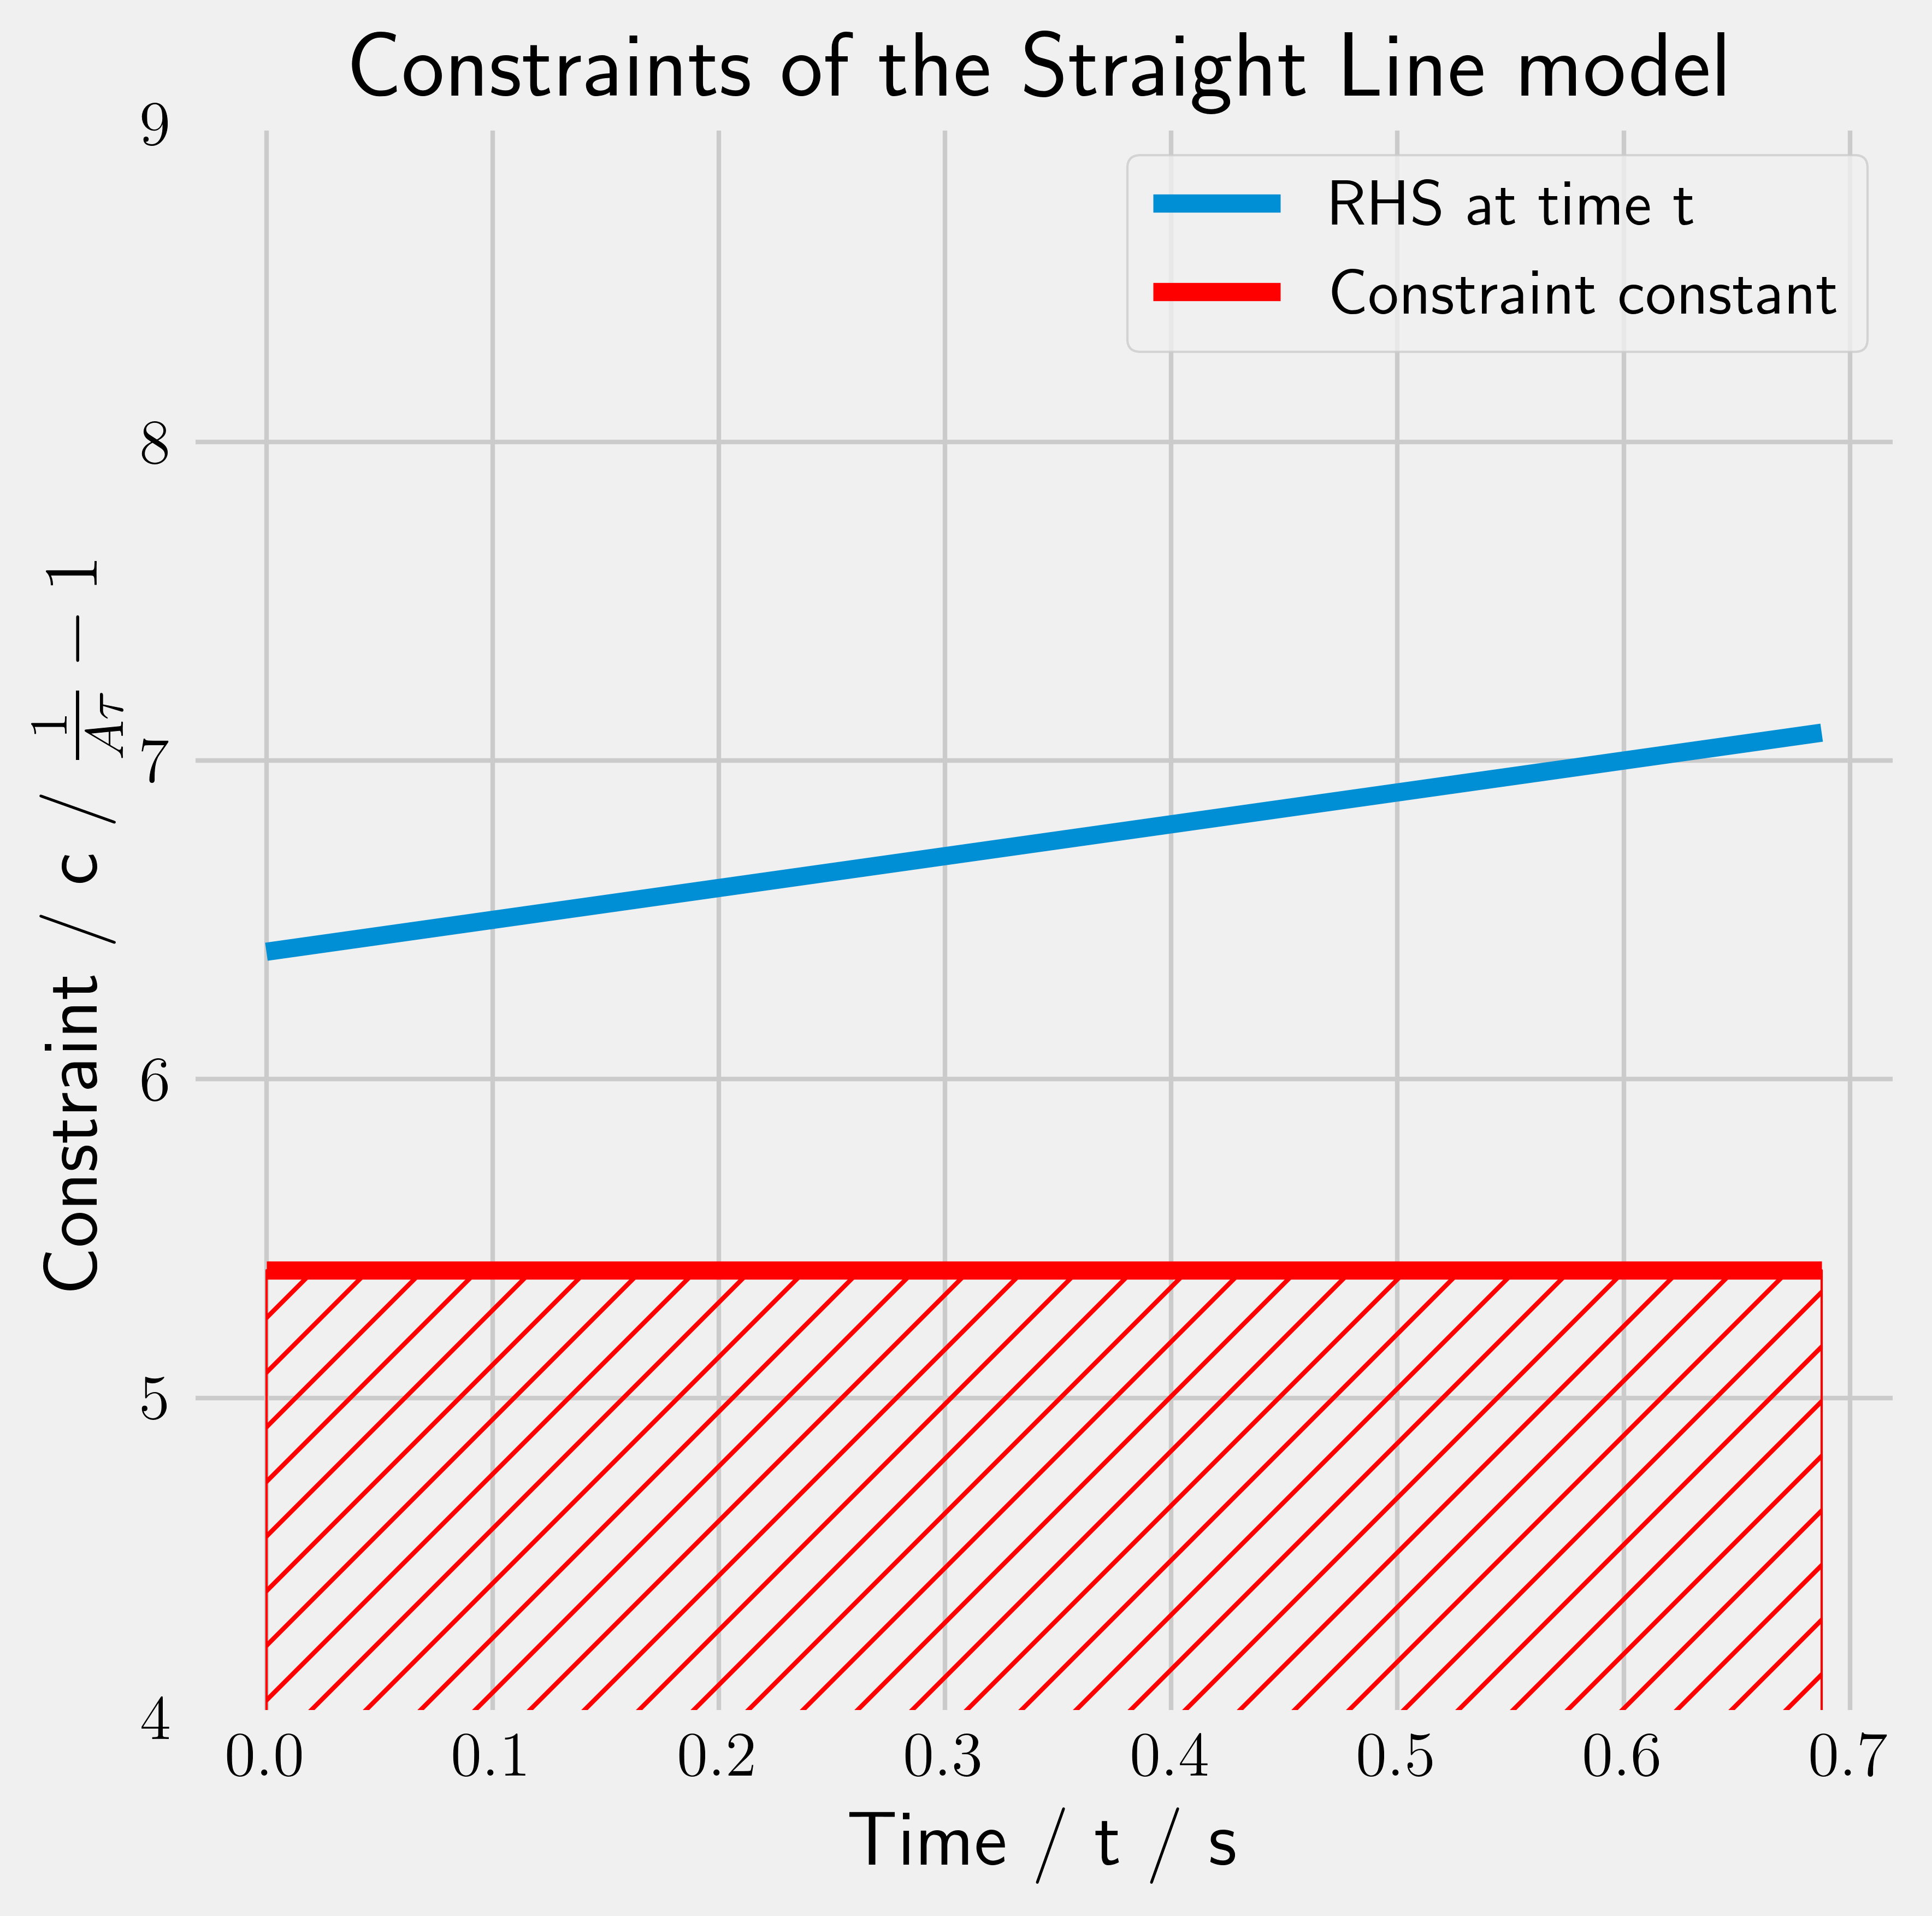
\includegraphics[width=0.45\textwidth,right]{assets/straight_constraint_inequality.png}
    \caption{}
    \label{fig:straight_constraint_inequality}
\end{wrapfigure}

But the game analyzed does have the constraint of a speed limit so players cannot accelerate infinitely, traveling across the map in two-to-three seconds. The graphing of the constraint (equation \ref{eq:constraint}) shows the problems (figure \ref{fig:straight_constraint_inequality}).

It is obvious that the RHS (top line) is higher than the constraint LHS (bottom shaded area). This indicates that the player exceeds the speed limit for every time within the considered time domain, which will undoubtedly massively decrease the restricted displacement. The inequality of the RHS can be represented symbolically by substitution of the player acceleration function into equation \ref{eq:constraint}:
\[
    5.4 \ge t + \frac{v_{0y}}{w}.
\]

Because the variable $\frac{v_{0y}}{w} = 6.4$, the inequality will only hold in negative $t$, which is not in the time domain considered. Only when the initial y-axis velocity is below $\frac{5.4 w}{v_{0y}}$ would there be acceleration on the first frame.

Therefore the restricted player motion would be without any acceleration at any time. The continuous displacement of the player at time $t_f$ can be computed by setting the variable $w=0$, or:
\begin{align*}
 \tp(t)_x &= t v_{0x} = 0\\
 \tp(t)_y &= t v_{0y}\\
 \tp(t_f)_y &= 0.7 \times 250 = 175.
\end{align*}

The discrete restricted jumping equation using Euler's method (figure \ref{eq:rje}) resulted in a similar distance of $175.78$, using constant $h=\tau$. Furthermore I've noticed that the displacement/time graph (figure \ref{fig:straight_constraint}) have displacements equality spaced in the y-axis --- in contrast with the ever expanding dots in the unrestricted case (figure \ref{fig:straight_nothing_1}). I believe that this indicates a lack of acceleration, which greatly reduced the result of this baseline model. Furthermore, the lack of acceleration means that this model can also be achieved with no player inputs, as the minimum value of acceleration $w$ is zero.

\begin{wrapfigure}{r}{0.48\textwidth}
    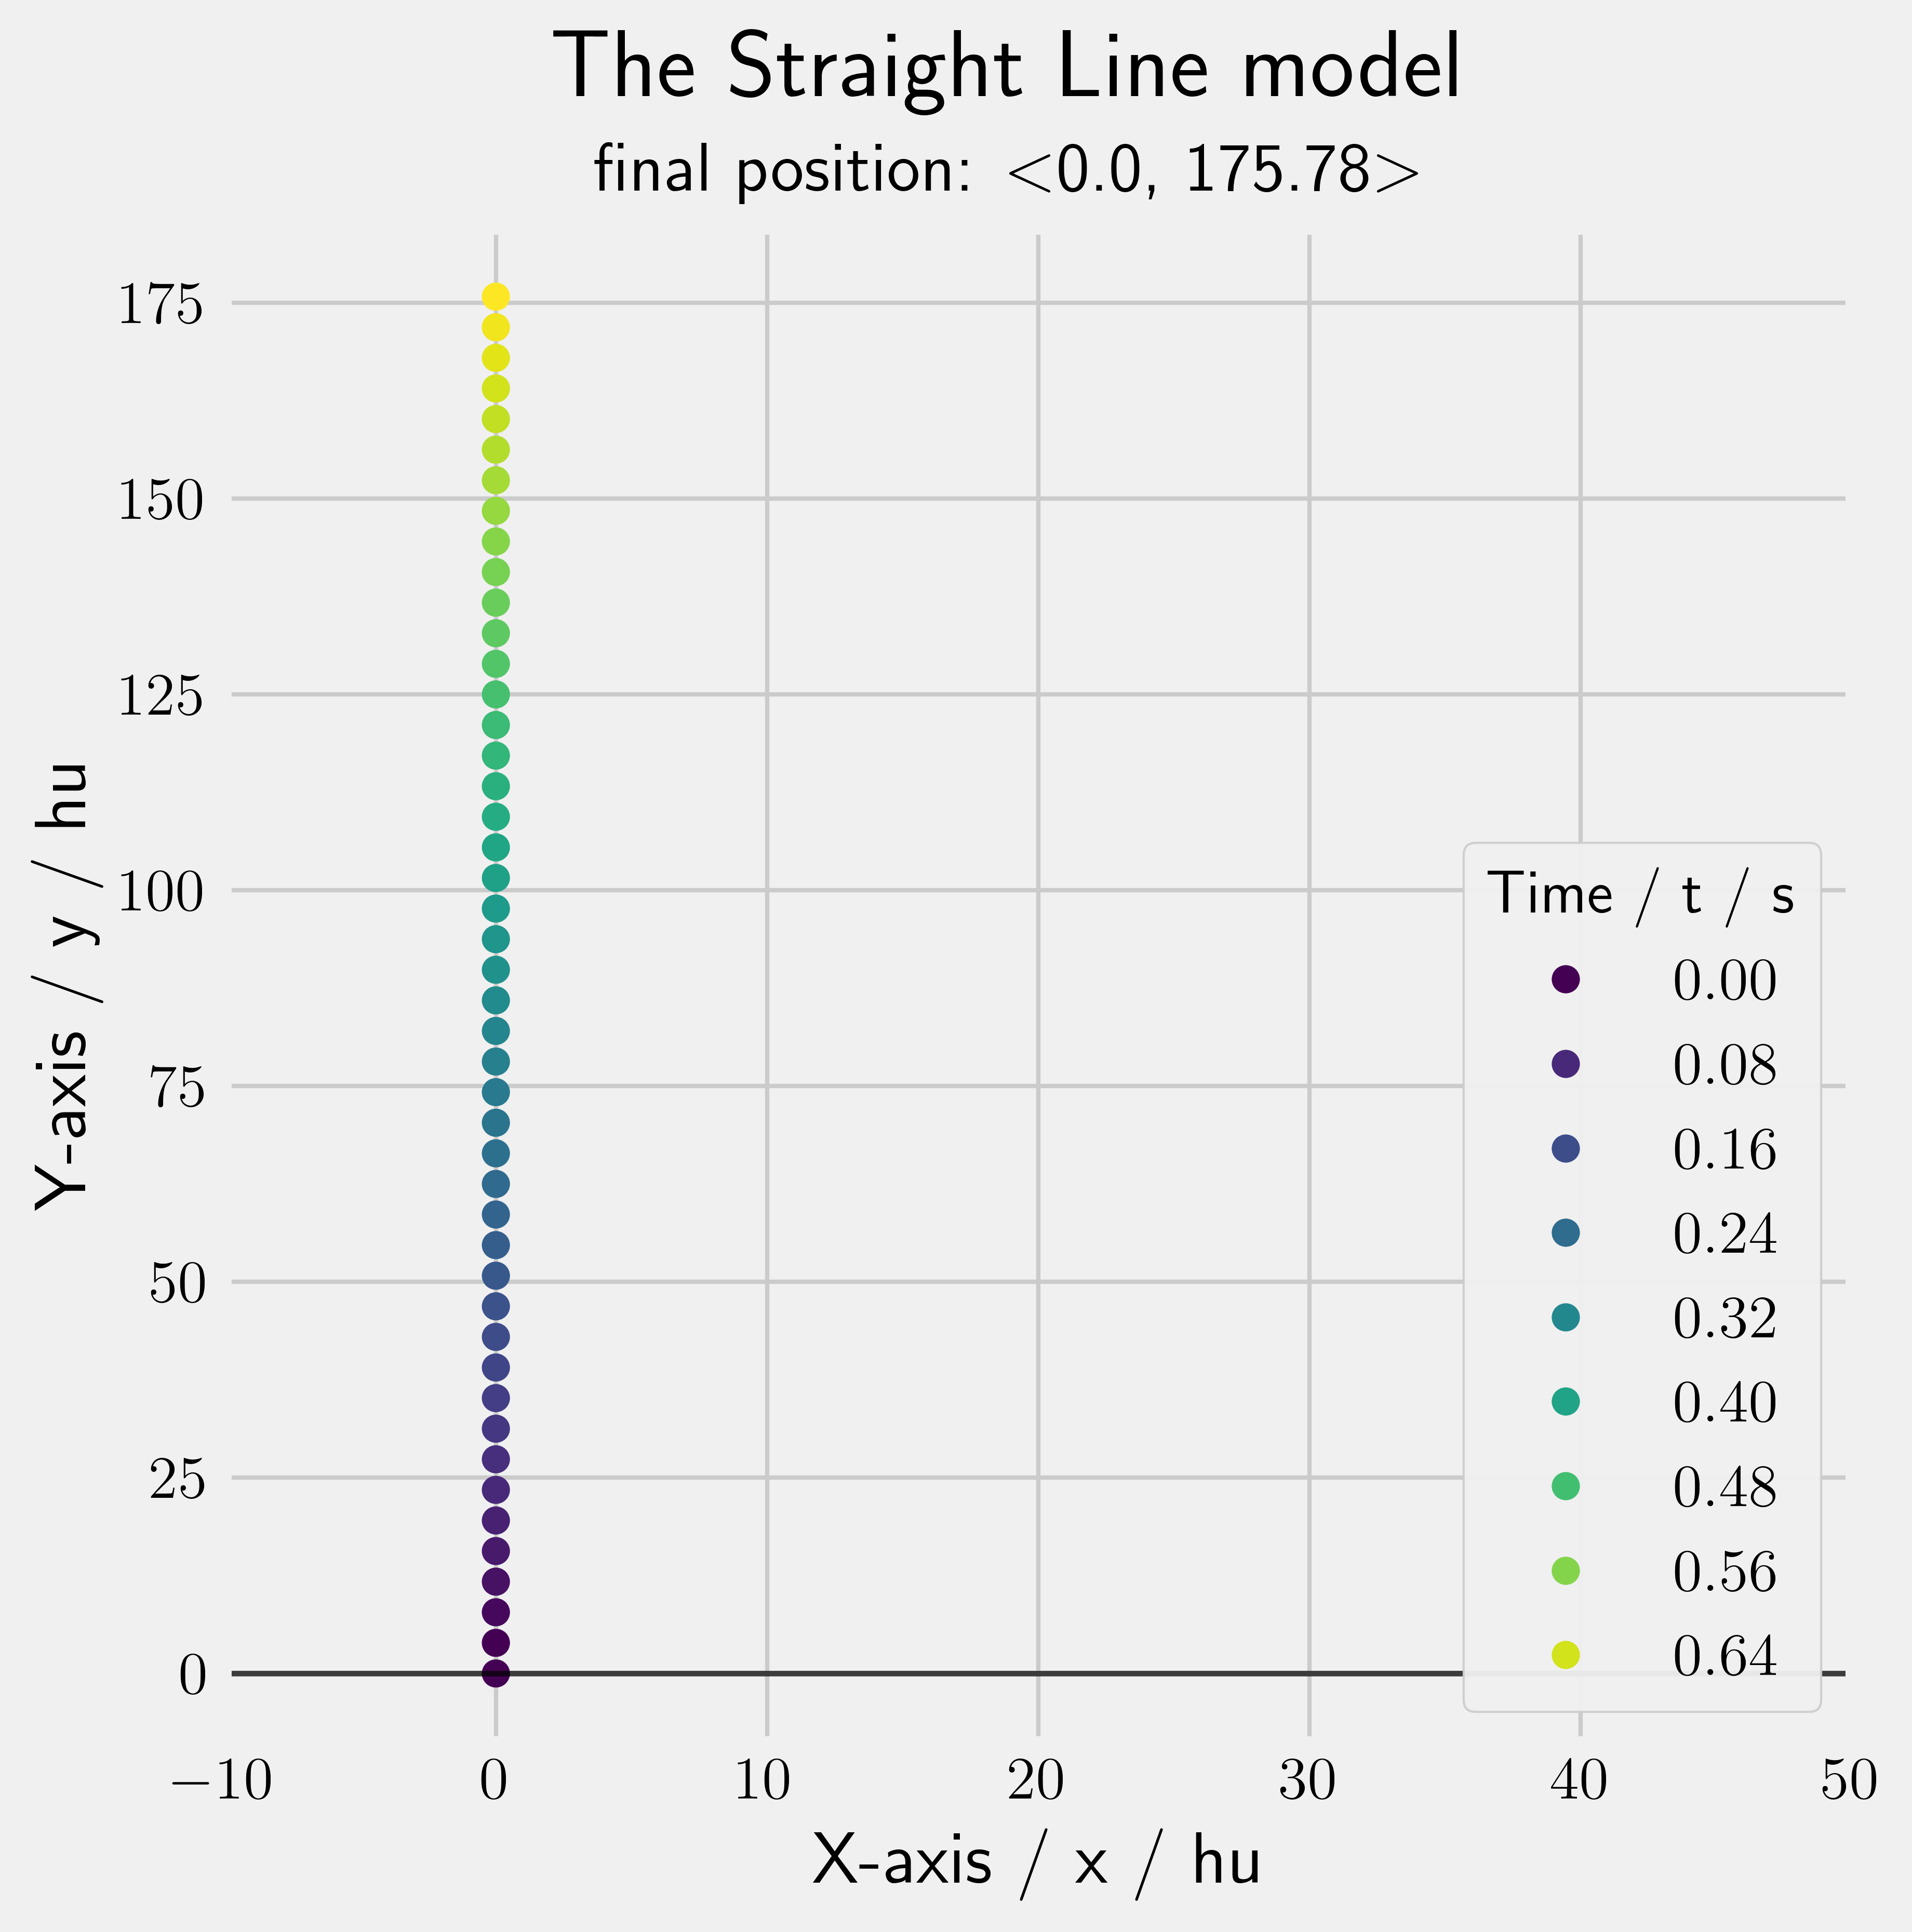
\includegraphics[width=0.45\textwidth,right]{assets/straight_constraint.png}
    \caption{}
    \label{fig:straight_constraint}
\end{wrapfigure}

Overall, the straight-line model establishes the baseline of my analysis. Using this strategy, the player has traveled an average distance in a jump of around $175$ hammerunits, which is well below what I can achieve in-game. The method has the benefit of requiring no input from the player, and can be performed consistently every  time. This makes the method the best model to conserve human energy by minimizing the amount of effort. But we can do better.

% conclusion

% Do not have enough words for this machine learning step
%\subsection{Machine learning}
%To kick start the optimization step, I decided to utilize the computing power I have access to to run a machine learning model on this problem. The result of which can potentially be graphed and fitted a model against, which could potentially be optimized further.

%From my previous experience in strafing sub-optimally, I hypothesize that

% state the steps of this

\subsection{Step by step}


\subsection{Euler-Lagrange optimization}


% TODO: calculated the restricted line,

% TODO: conclude this: max 250 total words

% TODO Have around 1500 words

% 500 words each for each method

% 500 for conclusion

Do the step by step one

Do the euler-lagrange one

Extension, find the optimal angle for each

